\documentclass[letterpaper,12pt,]{article}

\usepackage[%
    left=1in,%
    right=1in,%
    top=1in,%
    bottom=1.0in,%
    paperheight=11in,%
    paperwidth=8.5in%
]{geometry}%

\usepackage{listings}
\usepackage{graphicx}
\usepackage{amsmath}
\usepackage[font=small,skip=-2pt]{caption}
\usepackage{subcaption}
\usepackage{hyperref}
\usepackage{booktabs}
\usepackage{pdfpages}
\usepackage{pgffor}
\usepackage[section]{placeins}


\lstdefinestyle{mystyle}{
    %backgroundcolor=\color{backcolour},
    %commentstyle=\color{codegreen},
    %keywordstyle=\color{magenta},
    %numberstyle=\tiny\color{codegray},
    %stringstyle=\color{codepurple},
    basicstyle=\footnotesize,
    breakatwhitespace=false,
    breaklines=true,
    captionpos=b,
    keepspaces=true,
    numbers=left,
    numberstyle=\footnotesize,
    stepnumber=1,
    numbersep=5pt,
    showspaces=false,
    showstringspaces=false,
    showtabs=false,
    tabsize=2,
    frame=single
}
\lstset{frame=single}

\pagestyle{empty} % Remove page numbering
\linespread{1.5} % Line Spacing

\begin{document}

\begin{titlepage}

\newcommand{\HRule}{\rule{\linewidth}{0.5mm}} % Defines a new command for the horizontal lines, change thickness here

\center % Center everything on the page
 
%----------------------------------------------------------------------------------------
%	HEADING SECTIONS
%----------------------------------------------------------------------------------------


\textsc{\LARGE McGill University}\\[3.5cm]
\textsc{\Large Computational Aerodynamics}\\[0.5cm] 
\textsc{\large MECH 539}\\[2.5cm]

%----------------------------------------------------------------------------------------
%	TITLE SECTION
%----------------------------------------------------------------------------------------

{ \huge \bfseries Final Project}\\[1.5cm] % Title of your document

\HRule \\[0.4cm]
%----------------------------------------------------------------------------------------
%	AUTHOR SECTION
%----------------------------------------------------------------------------------------

\begin{minipage}{0.4\textwidth}
\begin{flushleft} \large
\emph{Name:}\\
Doug \textsc{Shi-Dong} % Your name
\end{flushleft}
\end{minipage}
~
\begin{minipage}{0.4\textwidth}
\begin{flushright} \large
\emph{Student ID:} \\
260466662\\
\end{flushright}
\end{minipage}\\[4cm]

\vfill{}
{\large April 29, 2016}\\[2cm]

\end{titlepage}


\section{Scalar Dissipation - Euler Explicit}

A Euler Explicit (EE), Scalar Dissipation (SD) of 0.06 and CFL of 0.1 has been used.
Figure \ref{fig:q1p}-\ref{fig:q1c} shows the pressure distribution, the Mach number distribution and density residual convergence plot.

The exit static pressure is the same as it was initially assigned ($0.80p_{t_{in}}$) since the flow stayed subsonic. The flow accelerates in the converging nozzle and decelerates in the diverging part. Pressure drops as the flow accelerates and increases when it decelerates.

The convergence could have been faster with a higher CFL, but the same scalar dissipation and CFL was used as in Question 2 for the sake of simplicity.

\begin{figure}[!ht]
    \centering
    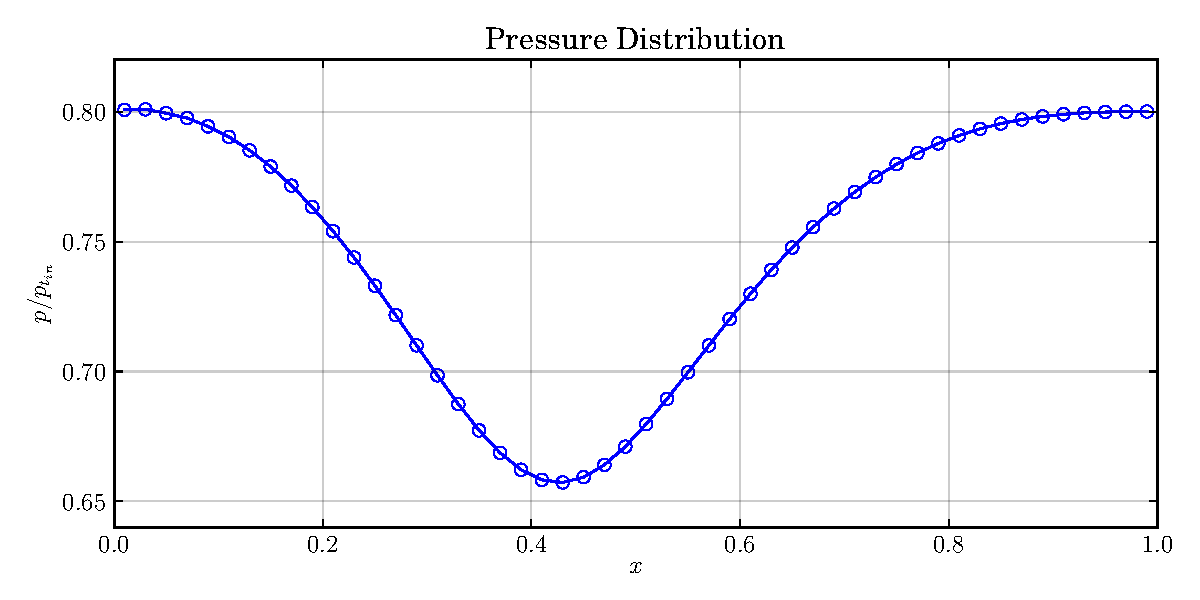
\includegraphics[width = 0.9\textwidth]{./figures/q1p.pdf}
    \caption {Pressure Distribution}
    \label{fig:q1p}
\end{figure}

\begin{figure}[!ht]
    \centering
    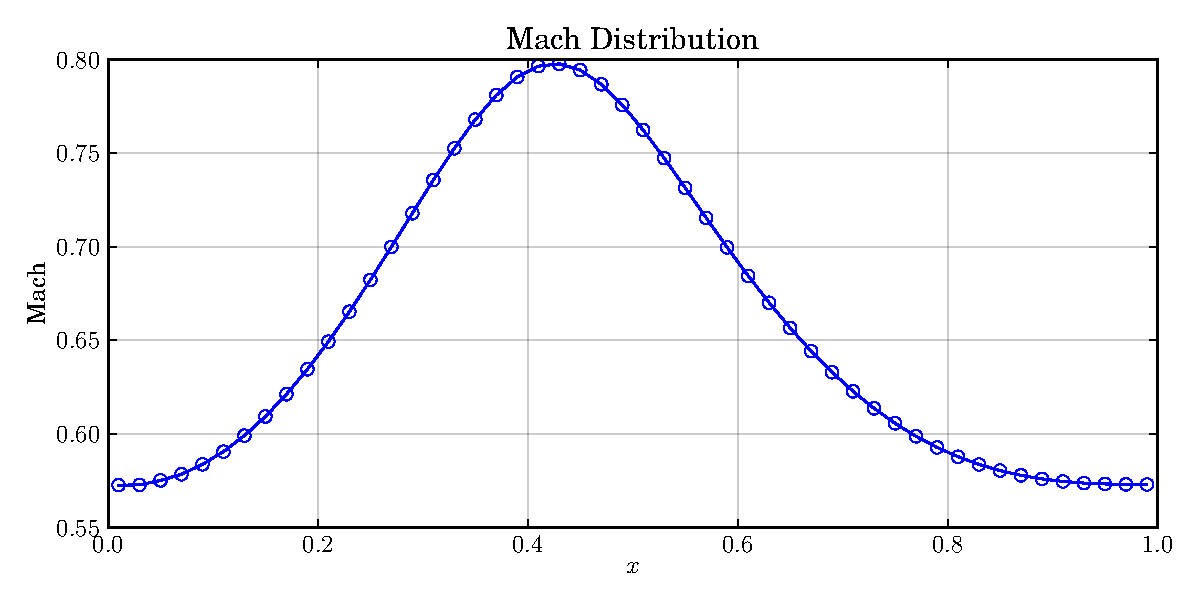
\includegraphics[width = 0.9\textwidth]{./figures/q1m.pdf}
    \caption {Mach Distribution}
    \label{fig:q1m}
\end{figure}

\begin{figure}[!ht]
    \centering
    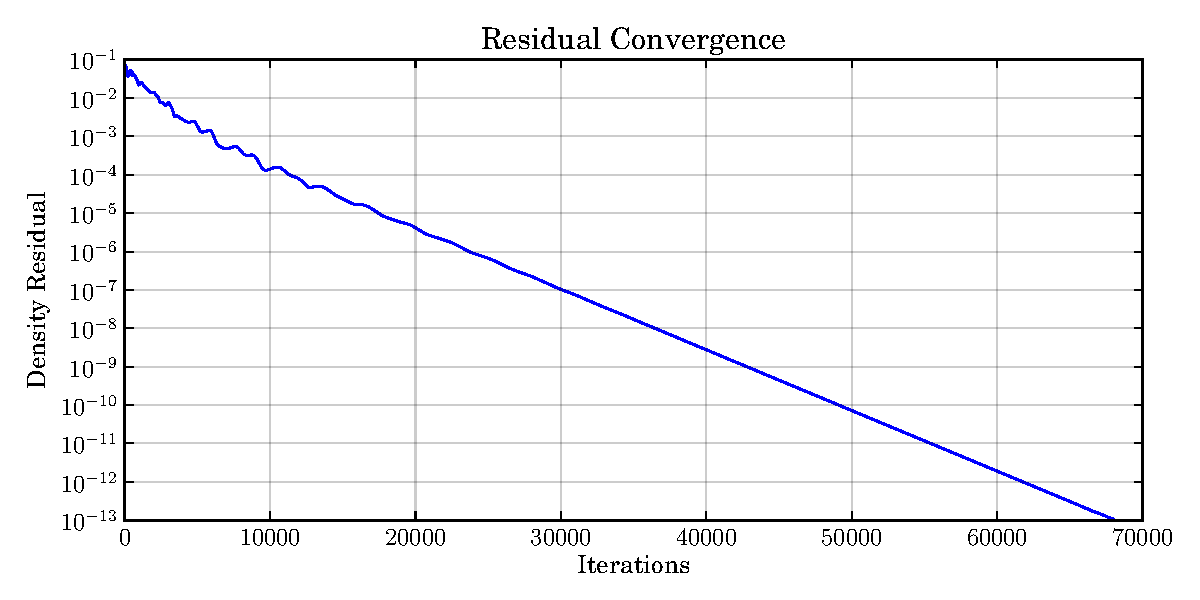
\includegraphics[width = 0.9\textwidth]{./figures/q1c.pdf}
    \caption {Density Residual Convergence}
    \label{fig:q1c}
\end{figure}

\section{Exit Pressure Study}

In order to retrieve a sharp shock with two points, a scalar dissipation of 0.06 was required.
Since the scalar dissipation from the scheme was relatively low, a lower CFL had to be used in order to prevent the algorithm from diverging.
A CFL of 0.1 was required to allow convergence.

Note that the CFL will not change the final solution, but the scalar dissipation parameter from the SD flux scheme will.
An EE time-stepping scheme should allow for an upper CFL of 1.0.
Reducing the CFL allows to dissipate some energy between each time step, whereas reducing the scalar dissipation affects the energy dissipation in the steady-state solution.

For all 4 cases, a CFL of 0.1 allowed the scalar dissipation of 0.06 to converge.
If a higher CFL was desired, the code would probably not be stable for this scalar dissipation parameter in all 4 cases.

Figure \ref{fig:q1p}-\ref{fig:q1c} shows the pressure distribution, the Mach number distribution and density residual convergence plot for various exit pressures.

\begin{figure}[!ht]
    \centering
    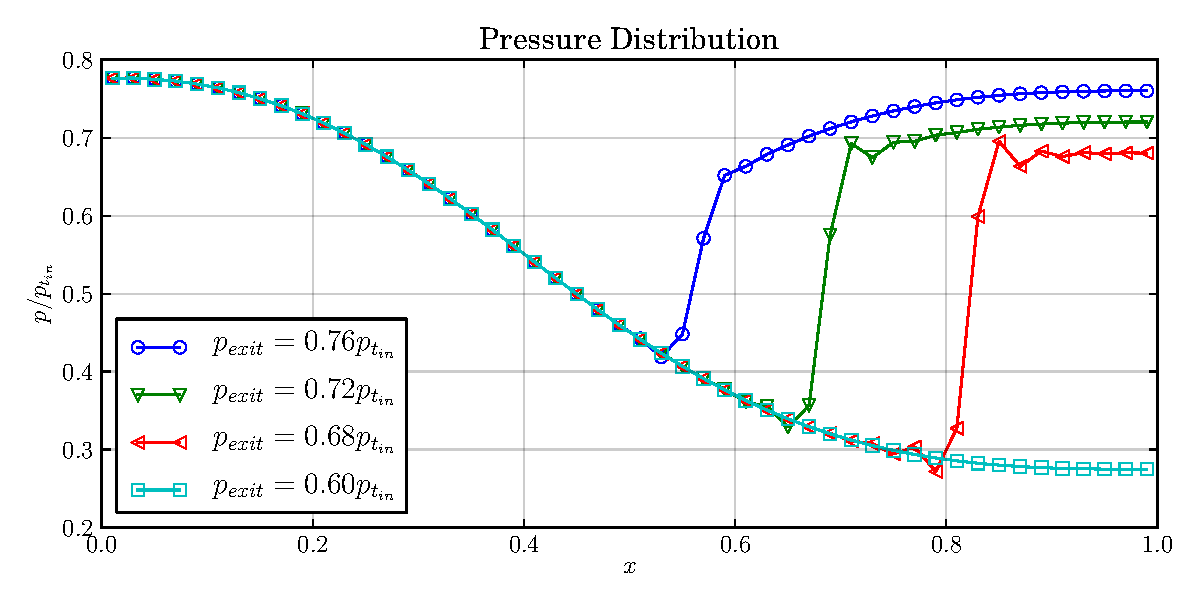
\includegraphics[width = 0.9\textwidth]{./figures/q2p.pdf}
    \caption {Pressure Distribution for Various Exit Pressures}
    \label{fig:q2p}
\end{figure}

\begin{figure}[!ht]
    \centering
    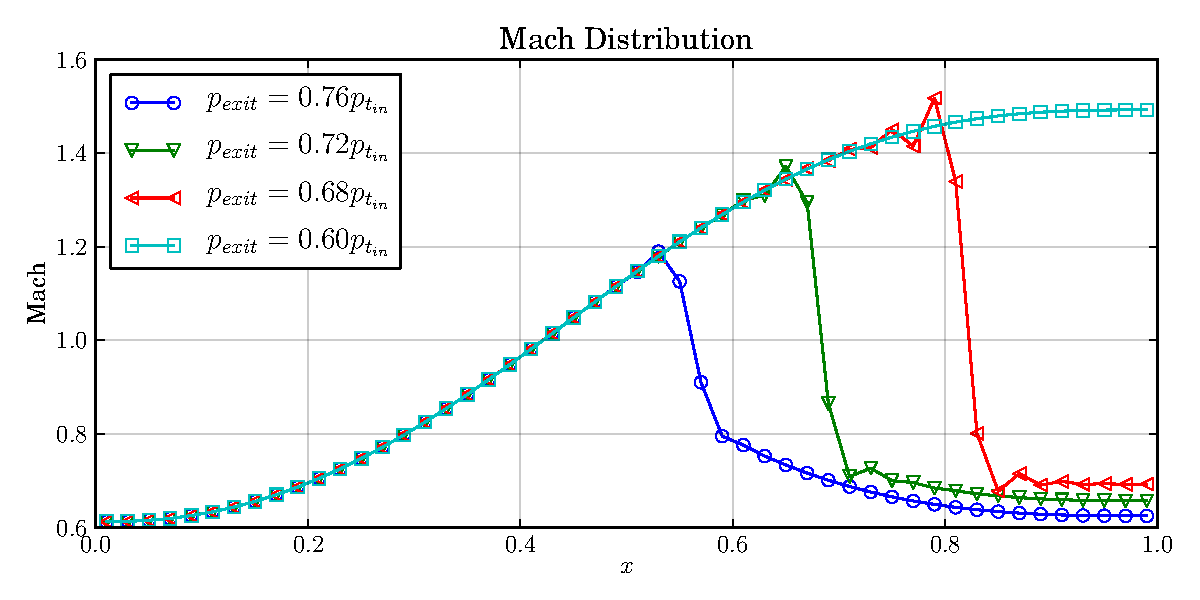
\includegraphics[width = 0.9\textwidth]{./figures/q2m.pdf}
    \caption {Mach Distribution for Various Exit Pressures}
    \label{fig:q2m}
\end{figure}

An exit static pressure of $0.76p_{t_{in}}$ exhibits a relatively small shock.
Before the throat, the flow is subsonic and accelerates in the converging nozzle.
At the throat, the flow is chocked and sonic.
In the diverging nozzle, the flow accelerates since it is now supersonic until the shock occurs.

As the back-pressure decreases, the shock moves towards the exit and becomes stronger because the flow must retrieve the exit static pressure.
The solution before the shock completely overlaps since no information can travel to the left in the supersonic region.

For an exit static pressure of $0.60p_{t_{in}}$, the flow past the throat is fully supersonic.
Since the exit is supersonic, only right-moving characteristics may influence the outlet, which means that the exit static pressure depends on everything on the left only.
The static pressure does not retrieve the back-pressure inside the channel but a Prandtl-Meyer expansion would be expected outside the channel.

\begin{figure}[!ht]
    \centering
    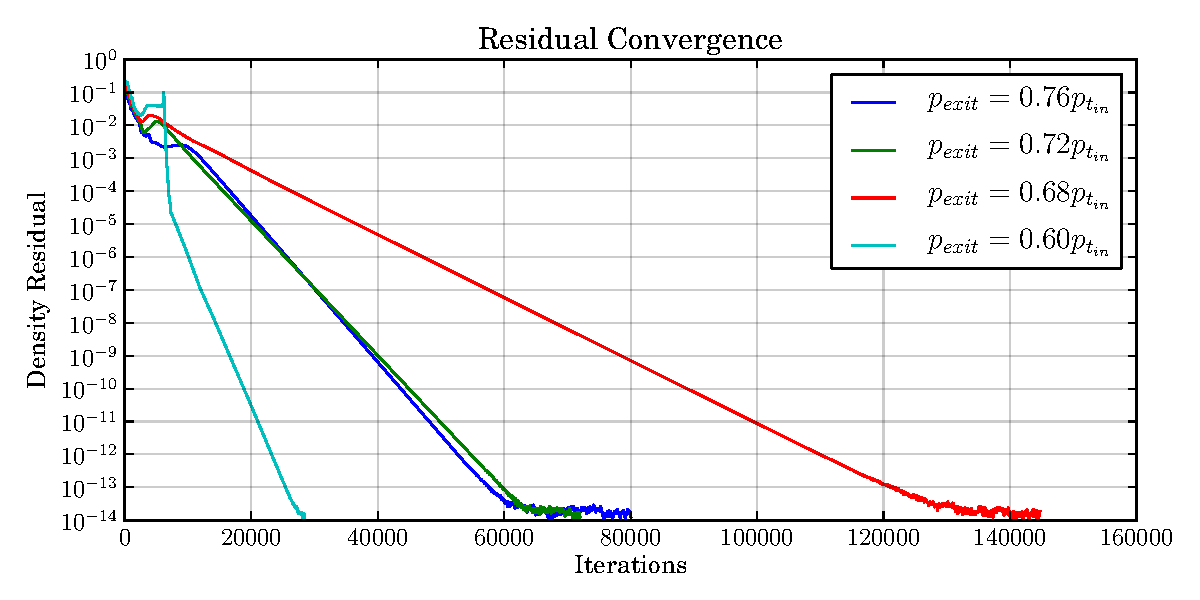
\includegraphics[width = 0.9\textwidth]{./figures/q2c.pdf}
    \caption {Density Residual Convergence for Various Exit Pressures}
    \label{fig:q2c}
\end{figure}

Numerically, it seems that the strongest shock for a back-pressure of $0.68p_{t_{in}}$ required many more iterations to converge, whereas the shock-free flow required less iterations to converge.
Resolving a shock might be harder due to the presence of large changes in the flow.

\section{Grid Study}

For the grid study, EE and SD with a CFL of 0.1 and $\epsilon = 0.06$.
Figure \ref{fig:q3p}-\ref{fig:q3c} shows the pressure distribution, the Mach number distribution and density residual convergence plot for various exit pressures.

\begin{figure}[!ht]
    \centering
    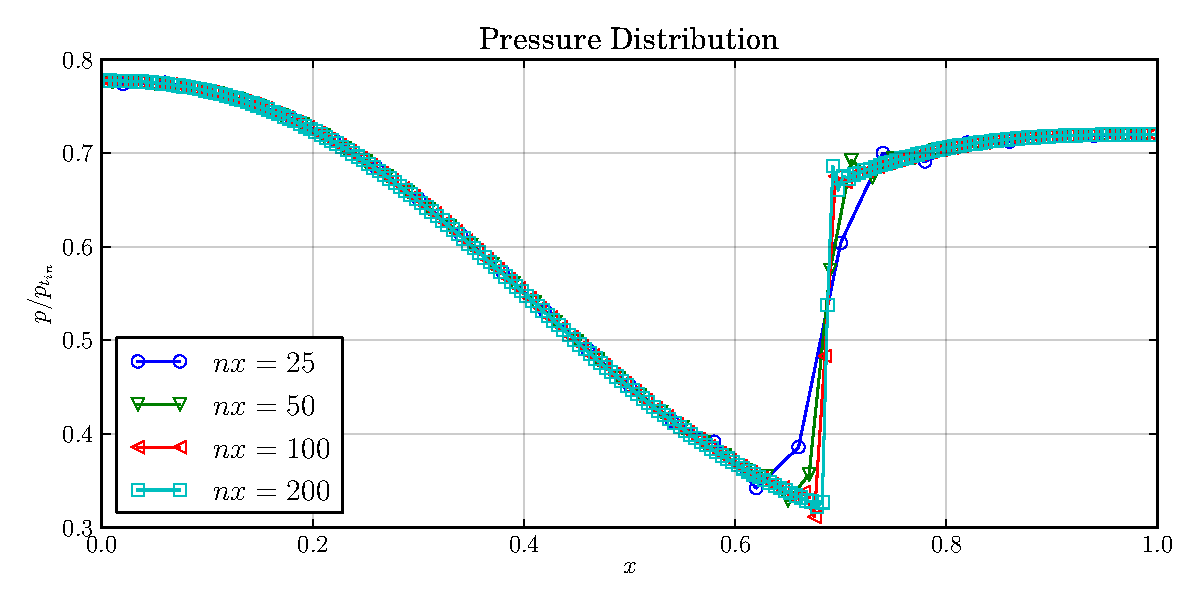
\includegraphics[width = 0.9\textwidth]{./figures/q3p.pdf}
    \caption {Pressure Distribution for Various Grid Sizes}
    \label{fig:q3p}
\end{figure}

\begin{figure}[!ht]
    \centering
    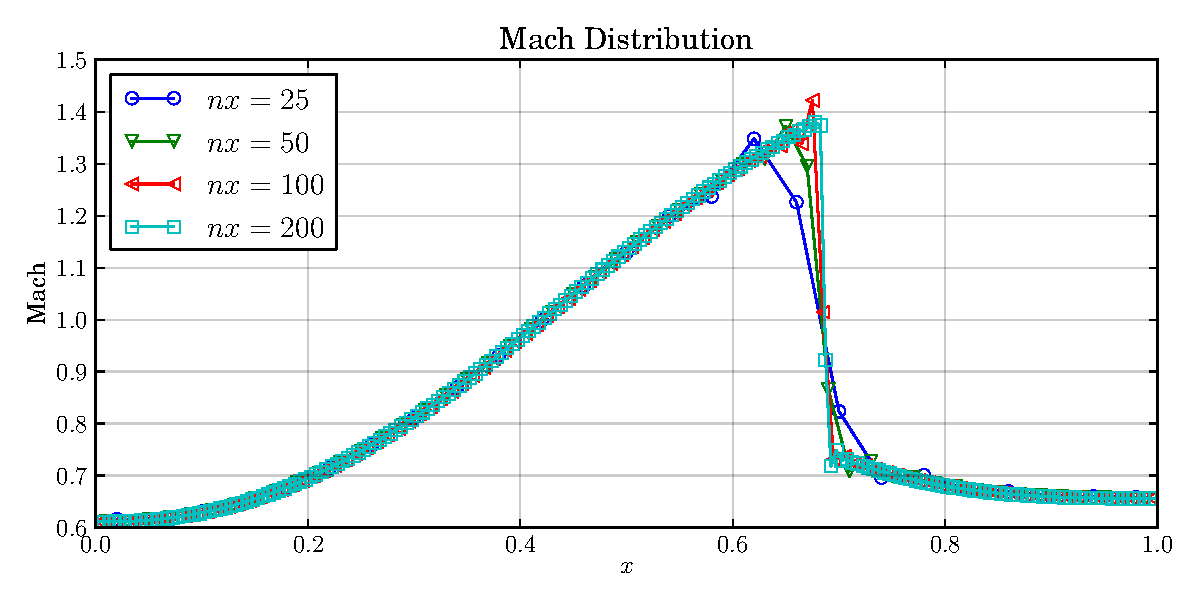
\includegraphics[width = 0.9\textwidth]{./figures/q3m.pdf}
    \caption {Mach Distribution for Various Grid Sizes}
    \label{fig:q3m}
\end{figure}


All four grids (25, 50, 100, 200) have a shock at the same location.
The location of the shock should not change with the number of grid points.
In fact, the shock becomes more apparent and sharper as the grid resolution increases.

As the number of grid point increases $dx$ decreases and affects the time-steps taken.
The CFL number is defined as $CFL = \lambda(dt/dx)$.
Since the CFL cannot be increased above 1.0 for an EE scheme, the time-step $dt$ must vary proportionally to $dx$.
Therefore, a large grid entails a small $dx$, which leads to a small $dt$, causing a slower convergence.

\begin{figure}[!ht]
    \centering
    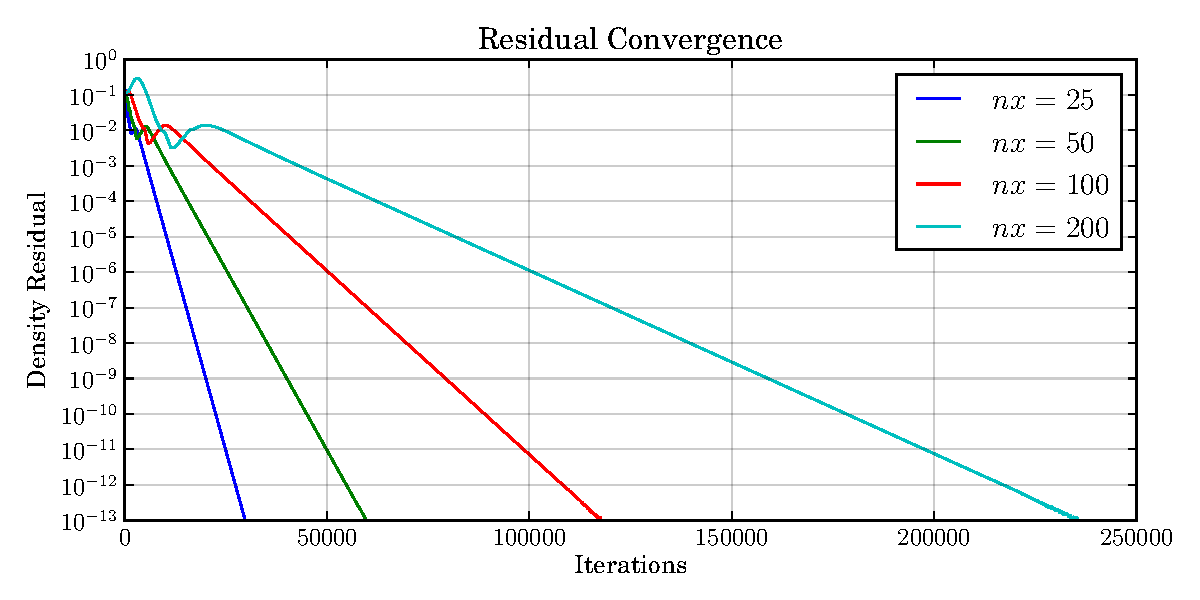
\includegraphics[width = 0.9\textwidth]{./figures/q3c.pdf}
    \caption {Density Residual Convergence for Various Grid Sizes}
    \label{fig:q3c}
\end{figure}

In fact, Figure \ref{fig:q3c} shows that the number of iterations required is almost exactly linearly proportional to the grid size.

Table \ref{tab1} shows the total pressure loss (TPL) for the various grid sizes and Figure \ref{fig:q3loss} shows the data on a plot.
A greater number of points increases the TPL because the shock is more accurately resolved.
As the number of points increases, the TPL should converge as seen in Figure \ref{fig:q3loss}.

\begin{figure}[!ht]
    \centering
    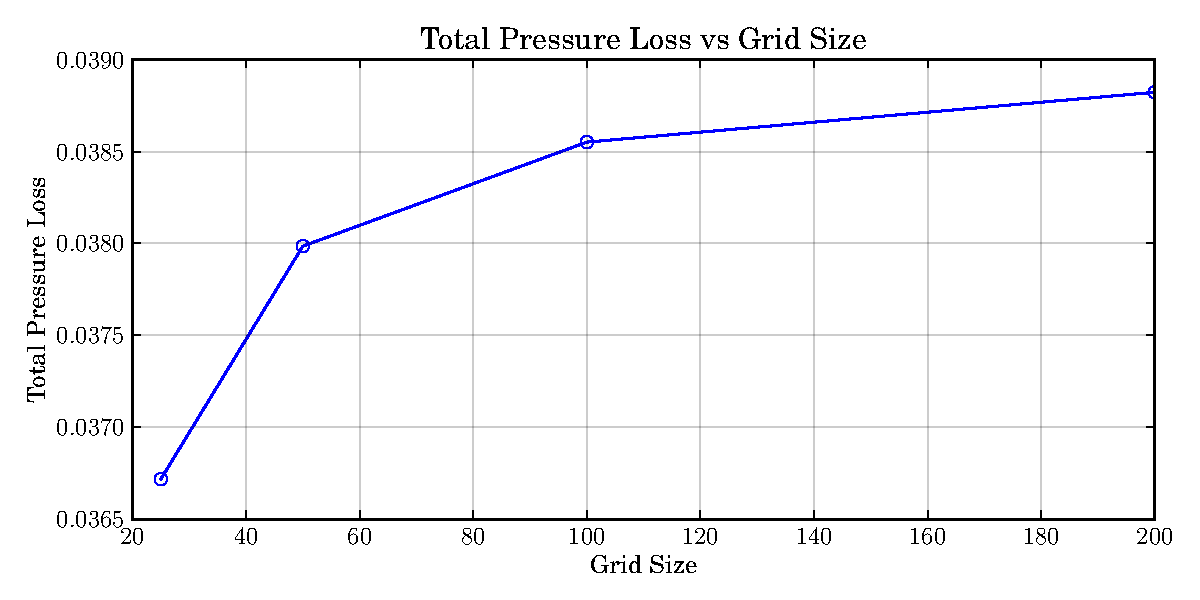
\includegraphics[width = 0.9\textwidth]{./figures/q3loss.pdf}
    \caption {Total Pressure Loss Grid Study}
    \label{fig:q3loss}
\end{figure}

\begin{table}[!h]
\centering
\begin{tabular}{cc} \toprule
    {Number of Grid Points} & {Total Pressure Loss} \\
    \midrule
    {25}  & 0.0367182\\
    {50}  & 0.0379852\\
    {100} & 0.0385511\\
    {200} & 0.0388222\\
\bottomrule
\end{tabular}
\caption{Total Pressure Loss for Various Grid Sizes}
\label{tab1}
\end{table}

\section{Flux Discretization Study}

For the flux discretization, EE with a CFL of 0.1 has been used.
Figure \ref{fig:q4p}-\ref{fig:q4c} shows the pressure distribution, the Mach number distribution and density residual convergence plot.
Scalar Dissipation (SD), Steger Warming (SW), CMSW (Corrected-Modified Steger-Warming) and Roe flux schemes are compared.

\begin{figure}[!ht]
    \centering
    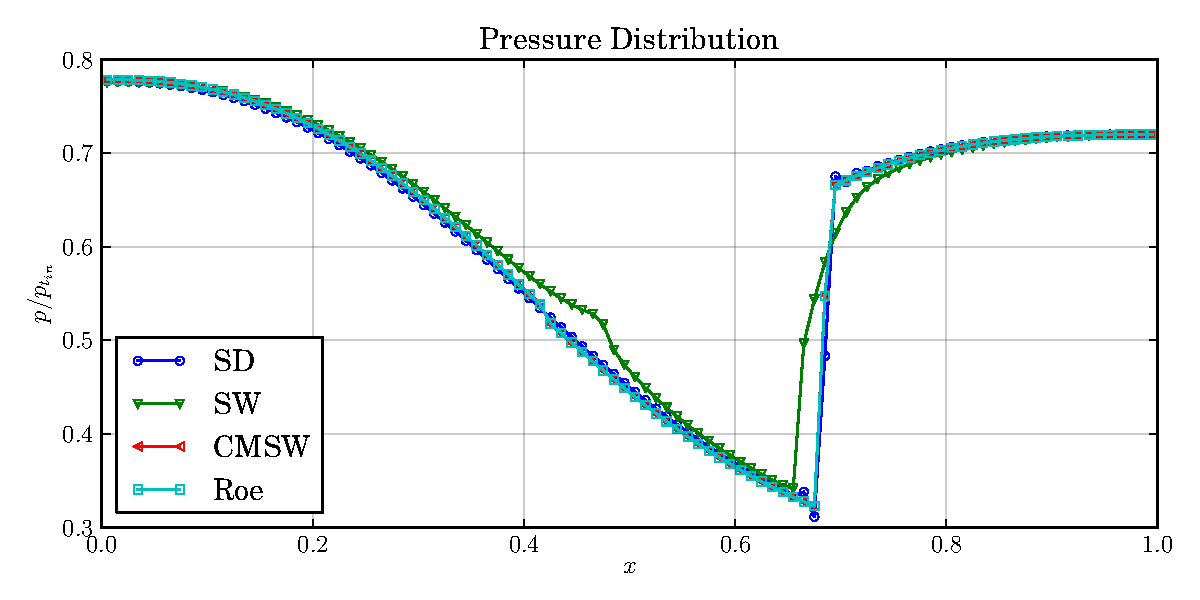
\includegraphics[width = 0.9\textwidth]{./figures/q4p.pdf}
    \caption {Pressure Distribution for Various Flux Schemes}
    \label{fig:q4p}
\end{figure}

\begin{figure}[!ht]
    \centering
    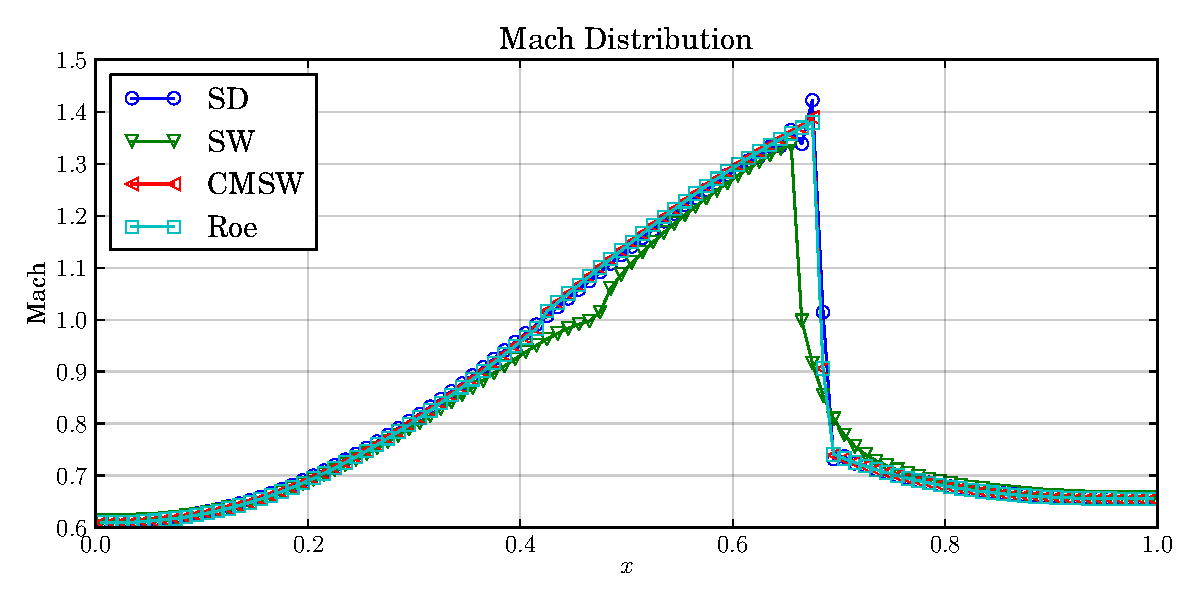
\includegraphics[width = 0.9\textwidth]{./figures/q4m.pdf}
    \caption {Mach Distribution for Various Flux Schemes}
    \label{fig:q4m}
\end{figure}
\begin{figure}[!ht]
    \centering
    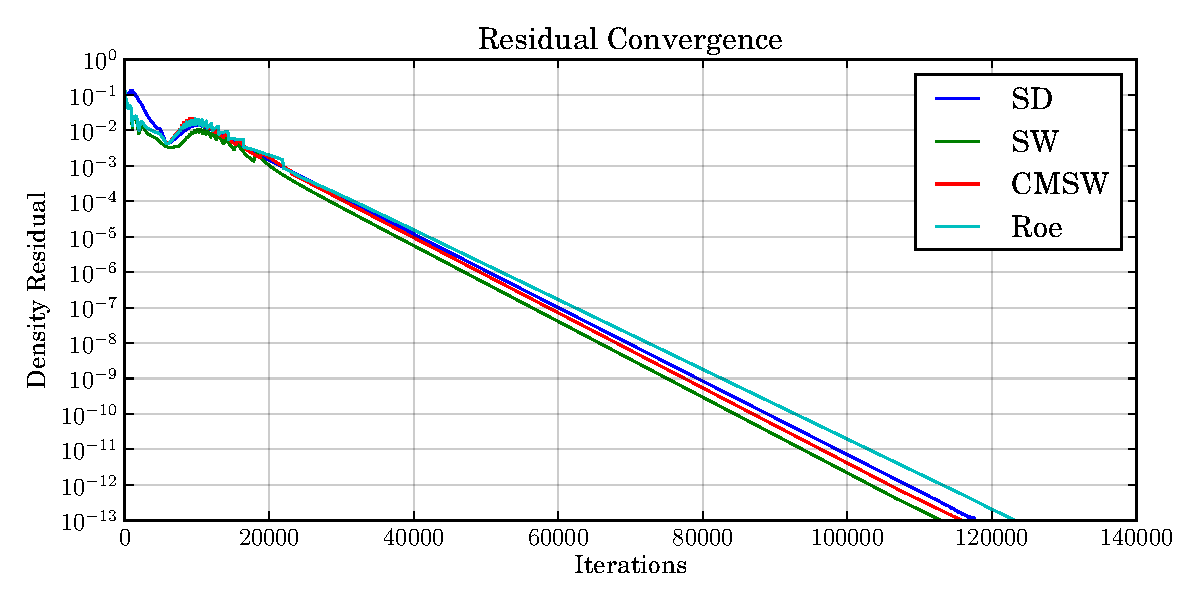
\includegraphics[width = 0.9\textwidth]{./figures/q4c.pdf}
    \caption {Density Residual Convergence for Various Flux Schemes}
    \label{fig:q4c}
\end{figure}


The solution slightly differs for the four difference flux schemes. SW differs the most in terms of solution.
Since SW is very dissipative, a weaker shock is required to match the exit pressure.
Therefore, the shock occurs earlier and is not at the same location as the other solutions.
The SW and CMSW also shows some oscillation at the sonic point since the fluxes are not continuously differentiable when the characteristic speeds are close to zero.
A larger blending $\epsilon$ would help alleviate the problem.
The SD scheme exhibits some dispersion at the shock which is probably due to the larger truncation error terms with odd derivatives.
The solution from Roe doesn't show any disadvantages in the solution since it captures the sonic condition and the shock without problems.

\begin{figure}[!ht]
    \centering
    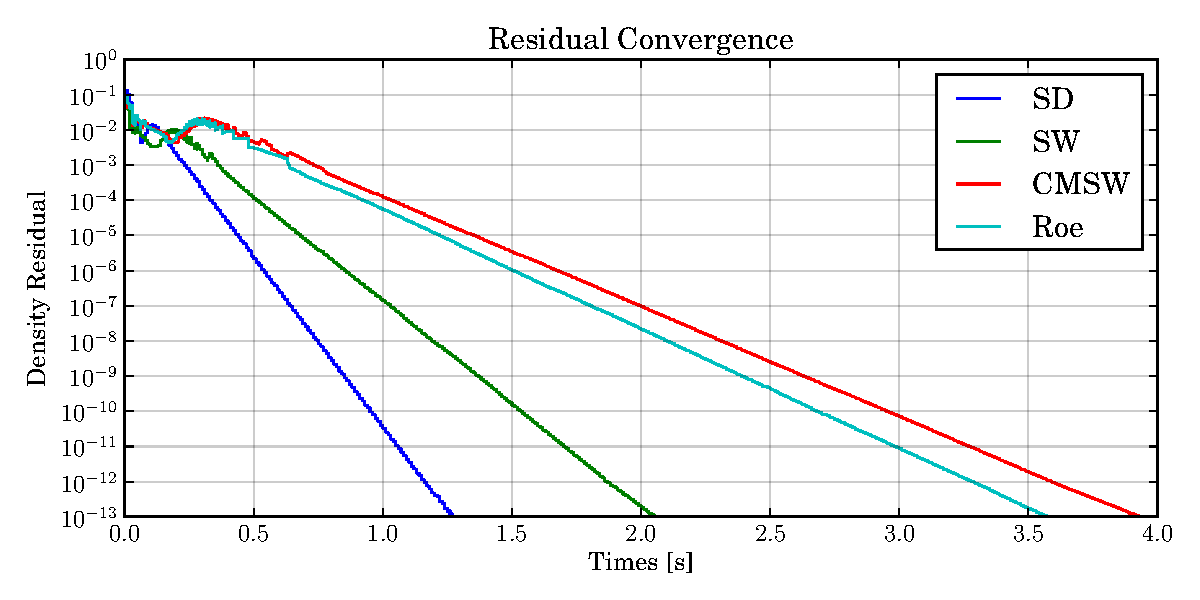
\includegraphics[width = 0.9\textwidth]{./figures/q4t.pdf}
    \caption {Density Residual Convergence versus CPU time for Various Flux Schemes}
    \label{fig:q4t}
\end{figure}


All four schemes take approximately the same number of iterations to converge. However, they do differ in terms of CPU time as shown in Figure \ref{fig:q4t}.
The SD scheme takes the least amount of time since less operations are required to retrieve the fluxes.
It is therefore a useful scheme since it is fast, easy to implement and gives a relatively accurate solution.
The SW scheme requires more time and is less accurate.
The CMSW corrects the dissipation problem, but at the cost of two SW flux evaluations, which means twice as much time.
Finally, Roe takes slightly less time than CMSW but does not suffer from the sonic oscillations of dispersion error at the shock.
It seems to give the solution with the least amount of numerical difficulties.

\begin{table}[!h]
\centering
\begin{tabular}{cc} \toprule
    {Flux Scheme} & {Total Pressure Loss} \\
    \midrule
    {SD}   & 0.0385511\\
    {SW}   & 0.0375229\\
    {MCSW} & 0.0395640\\
    {Roe}  & 0.0395788\\
\bottomrule
\end{tabular}
\caption{Total Pressure Loss for Various Flux Schemes}
\label{tab2}
\end{table}

Table \ref{tab2} shows the TPL for the different schemes.
Both CMSW and Roe retrieve the same TPL of 3.96\% where as SD and SW underestimate it.
The reason they underestimate the TPL could be explained by a weaker shock due to higher dissipation.
In a fully subsonic case, the TPL should be greater for SD and SW since the TPL would come from dissipation.

\section{Time Discretization Study}

For the time discretization study, Roe flux scheme is used for spatial discretization since the CFL does not need to be reduced to compensate for dissipation.
Euler-explicit (EE), Jameson's Runge-Kutta 4th order (JRK4) and Euler-Implicit (EI) schemes are compared.
The implicit scheme uses scalar dissipation since linearization is more straightforward.

Figure \ref{fig:q5p}-\ref{fig:q5m} shows the pressure distribution and the Mach number distribution.
The solution from the explicit schemes are exactly the same since the same flux discretization scheme is used.
Therefore, the time discretization should not affect the steady-state solution.

\begin{figure}[!ht]
    \centering
    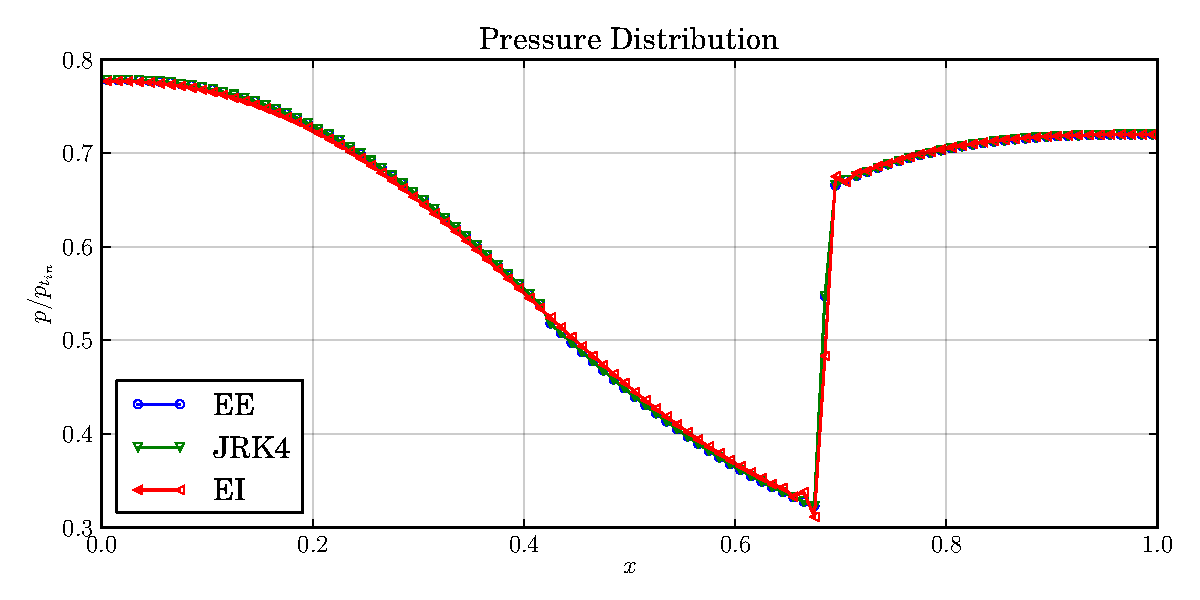
\includegraphics[width = 0.9\textwidth]{./figures/q5p.pdf}
    \caption {Pressure Distribution for Various Time-Stepping Schemes}
    \label{fig:q5p}
\end{figure}

\begin{figure}[!ht]
    \centering
    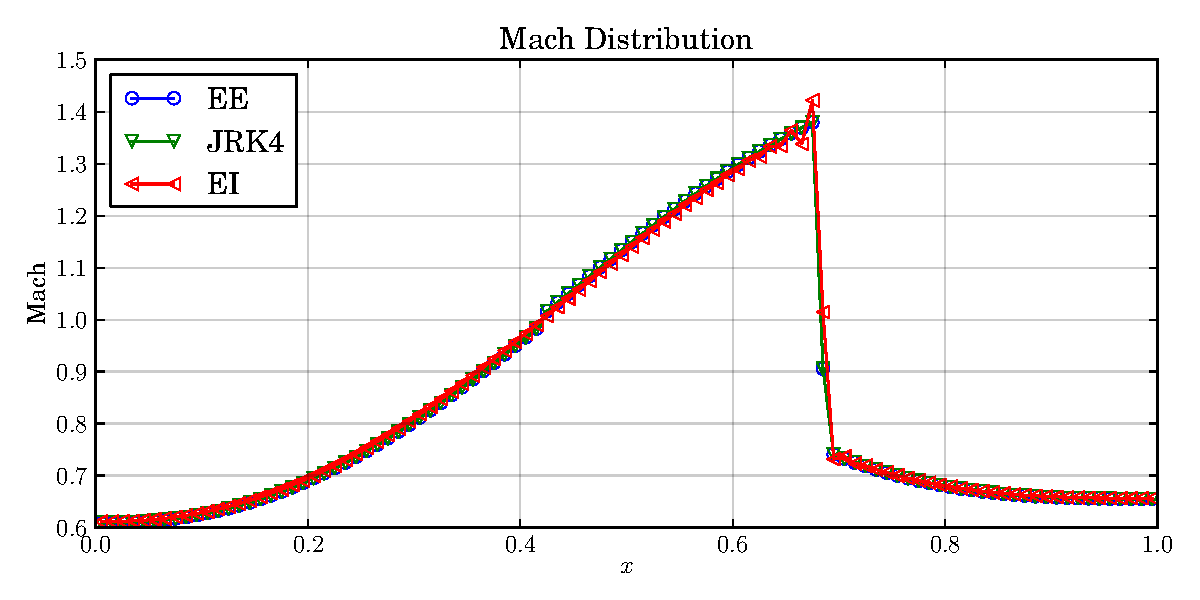
\includegraphics[width = 0.9\textwidth]{./figures/q5m.pdf}
    \caption {Mach Distribution for Various Time-Stepping Schemes}
    \label{fig:q5m}
\end{figure}

The difference between the time-stepping scheme appears when we start looking at the convergence in Figure \ref{fig:q5c} \& \ref{fig:q5t}.
Since the main goal of a more stable scheme is to allow for a higher CFL, the maximum stable CFL is used for each scheme.
Euler-explicit uses a CFL of 0.95.
JRK4 uses a CFL of 1.50.
Euler-implicit uses a variable CFL determined by the residual.
For every order of magnitude lower than 1.0\textsc{e}-2, the CFL grows cubically to finally reach a CFL of approximately 2000 at convergence.

The CFL number is directly linked to the number of iterations required to converge.
JRK4 is almost 1.5 times faster than EE with a CFL around 1.5 bigger.
However, every time-step requires more work since 4 pseudo-steps are done within the JRK4 iterations.
Therefore, in terms of CPU time, JRK4 should take 4/1.5 times longer than EE.
Figures \ref{fig:q5c} \& \ref{fig:q5t} show exactly the above in terms of iteration and CPU time.

The implicit scheme is harder to compare.
It requires considerably less iterations to converge since the CFL number grows cubically.
The CPU time is comparable to JRK4, however the comparison might not be fair for a few reasons.
The cost of assembling the matrix gives the implicit scheme a significant CPU time overhead.
This overhead have much less effect on a larger system of equation when solving for a full three-dimensional flow.
Also, the early iterations require a modest CFL to be used, losing the main advantage of implicit schemes and efficient way of increasing the CFL could be used.


\begin{figure}[!ht]
    \centering
    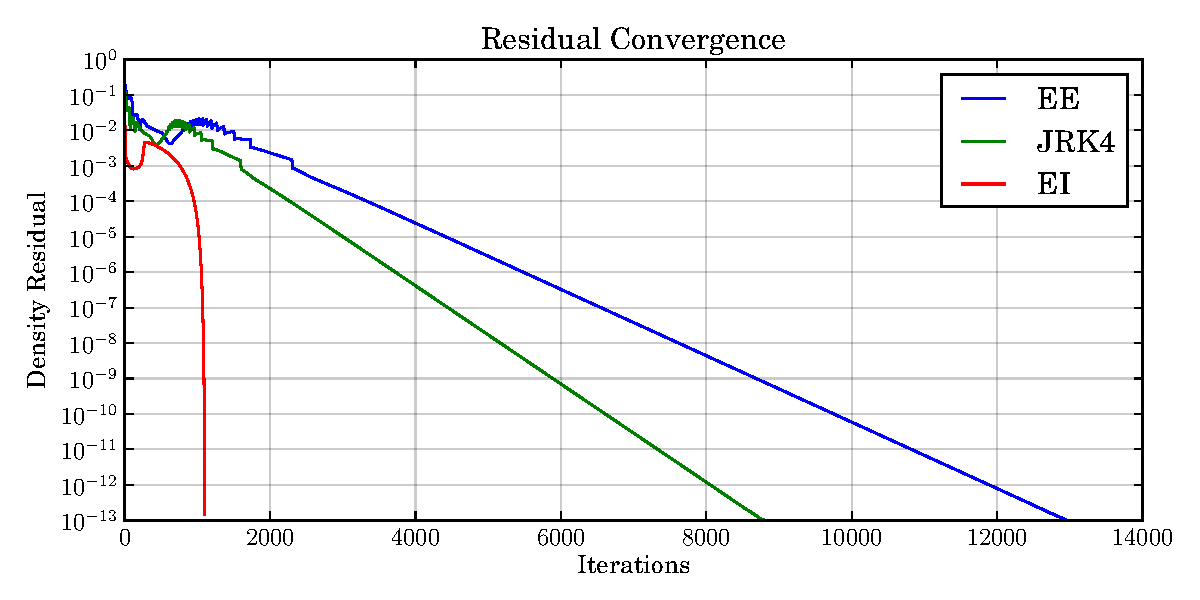
\includegraphics[width = 0.9\textwidth]{./figures/q5c.pdf}
    \caption {Density Residual Convergence for Various Time-Stepping Schemes}
    \label{fig:q5c}
\end{figure}

\begin{figure}[!ht]
    \centering
    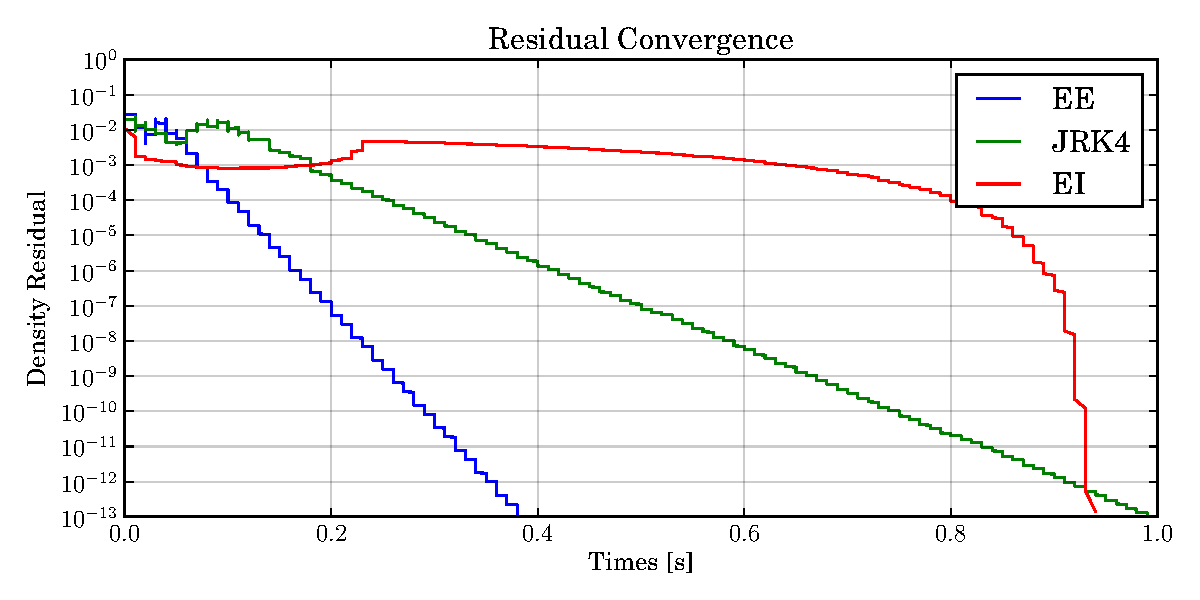
\includegraphics[width = 0.9\textwidth]{./figures/q5t.pdf}
    \caption {Density Residual Convergence versus CPU time for Various Time-Stepping Schemes}
    \label{fig:q5t}
\end{figure}

\section*{Codes}

Code has been written in C++ with optimization level -O3.

All codes are available on my GitHub:

\url{https://github.com/dougshidong/mech539/tree/master/final}

\end{document}
